\documentclass[]{article}
\usepackage[backend=biber, style=numeric]{biblatex}
\usepackage{paralist}
\usepackage{hyperref}
\usepackage{graphicx}
\usepackage{booktabs}
\usepackage{subcaption}
\usepackage{wrapfig}
\usepackage{float}

\graphicspath{ {./figures/} }
\usepackage{geometry}
\geometry{a4paper, portrait}

\addbibresource{report.bib}
\newtheorem{researchquestion}{RQ}

%opening
\title{Capita Selecta in Artificial Intelligence - Assignment 3}
\author{Arne Lescrauwaet \small(852617312) \and Joachim Verschelde \small(852594432) \and Alexander Van Hecke \small(852631385) \and Farid Rasoolzadeh Baghmisheh \small(852104522)}

\begin{document}

\maketitle

\section{Introduction} \label{sec:introduction}
This report details the step taken by Arne Lescrauwaet (852617312), Joachim Verschelde (852594432), Alexander Van Hecke (852631385) and Farid Rasoolzadeh Baghmisheh (852104522) for the assignment of the 2023/2024 Capita Selecta in Artificial Intelligence course organised by the Open University (\cite{ou}).

For this assignment we expand on the experiments described in \cite{durability}.
In this paper, the authors investigate the use of an LLM model and a RAG setup \cite{rag} to asses company durability disclosures.
By examining published sustainability reports of carbon-intensive companies, they investigate whether climate transition measures are disclosed in these reports.
A set of 64 indicators (questions) was used to investigate measures already taken or yet to be taken.
For each question, relevant passages in the published sustainability reports were retrieved and passed as additional context to the GPT-4 model.
Their main conclusions were :

\begin{itemize}
    \item Companies more often disclose information about measures yet to be taken (``Talk'' measures) than about measures that were already taken (``Walk'' measures).
    \item The RAG setup was judged by human experts and found to be mostly positive.
    \item An automated tool as developed by the authors can be a help to human experts, but are no replacements for human experts.
\end{itemize}

In this research, we want to expand on \cite{durability} in the following ways :

\begin{itemize}
    \item We examine data published by the fast fashion industry instead of carbon-intensive companies.
    \item We evaluate and compare several freely available LLM models instead of using a commercial LLM model.
    \item We evaluate additional indicators provided by dr. ir. Clara Maathuis of Open University \cite{ou}.
\end{itemize}

This research is related to the \textbf{text} cluster of the course \cite{ou}.
The text cluster introduces a number of techniques to improve the performance of LLM models for certain tasks.
One of the techniques discussed is RAG, first introduced in \cite{rag}.
RAG adds context when querying LLM models, allowing the model to get a better semantic understanding of the question and to generate a more relevant answer.
The main strenghts of a RAG based setup are \textbf{i)} the ability to access up-to-date information (no cutoff), \textbf{ii)} the ability to add domain specific knowledge, \textbf{iii)} efficiency, as the parameteric memory does not need to contain all knowledge and no retraining or fine-tuning is necessary, \textbf{iv)} the ability to generate more specific, more diverse and more factual answers and \textbf{v)} the scalability of the approach.
The main disadvantages of a RAG based setup include \textbf{i)} the context limits of LLM models, which restricts how much additional information can be passed, \textbf{ii)} the performance of the retriever as the weakest link in the setup, \textbf{iii)} the additional latency and complexity introduced, \textbf{iv)} the need to keep the knowledge base up-to-date.
Evaluation of climate transition disclosures presents an excellent concrete use case of RAG.

\section{Goal} \label{sec:goal}

\begin{quotation}
    discuss the objective of this project split it into multiple smaller objectives that will be tackled in this project
    \begin{itemize}
        \item Main goal
        \item Smaller objectives and report outline
    \end{itemize}
\end{quotation}

The goal of this assignment is to expand on the RAG setup introduced in \cite{durability}, by using different data, different LLM models and additional metrics.

Instead of focusing on carbon-intensive industry, we want to examine sustainability reports published by fast fashion companies.
This illustrates the ability of RAG based setups to easily incorporate domain specific knowledge or questions.
Section \ref{sec:data analysis} details the data used.

As described in \cite{durability}, the GPT-4 model performs well on the specific task of examining sustainability reports.
It is interesting to see how freely available models compare to commercial models.
Furthermore, we expand the initial set of 64 indicators by examining two additional scenarios.
In the first scenario \textit{(greenwashing detection)} we assess if a company shows potential signs of involvement or engagement with greenwashing methods and practices.
In the second scenario \textit{(greenwashing mitigation)} we provide relevant mitigation methods if the company is indeed engaging in greenwashing practices.
In section \ref{sec:methodology} we detail the models we evaluate and the experiments conducted.

Section \ref{sec:evaluation} details the evaluation of the results.
We do both a quantitative and a qualitative evaluation.
Since the LLM is asked to not only judge whether the question is true or false, but also to provide argumentation about the decision made, it is important to evaluate the argumentation.
Metrics such as coherence, consistency and relevance are important in this context.

Finally, we summarize the approach and provide conclusions in section \ref{sec:conclusions}.

\section{Data analysis} \label{sec:data analysis}

\begin{quotation}
    describe the dataset used considering entities such as features and target, and discuss processing and cleaning aspects like duplicates and outliers
    \begin{itemize}
        \item Dataset description
        \item Data processing
        \item Data cleaning
        \item Data visualization and interpretation
    \end{itemize}
\end{quotation}

For this assignment, we investigate the 2023 sustainability reports of two fast-fashion companies (\textbf{H\&M} and \textbf{Zara}).
There reports are publicly available in PDF format.
Since we use the \texttt{llama\_index} python package to extract the text from the PDF files, no additional data processing or cleaning is necessary.
The \texttt{SentenceSplitter} class is used to extract coherent text blocks from PDFs.
In order to keep sentences together as much as possible, we use a \texttt{chunk\_size} of 350, and a \texttt{chunk\_overlap} of 50.
We retrieve the 8 most relevant chunks as additional context for each question.

\section{Methodology and Implementation} \label{sec:methodology}

\begin{quotation}
    describe the followed methodological approach and discuss important implementation choices providing concrete examples
    \begin{itemize}
        \item Research Methodology discussion
        \item Design elaboration
        \item Implementation choices discussion
    \end{itemize}
\end{quotation}

\section{Evaluation and Results} \label{sec:evaluation}

% \begin{quotation}
%     discuss the evaluation method and criteria used, and interpret the results obtained considering both technical and ethical aspects (norms and values)
%     \begin{itemize}
%         \item Evaluation mechanism discussion and evaluation criteria selected
%         \item Results description using different data visualization methods.
%         \item Interpretation of the results obtained and positioning in the field considering both relevant technical and ethical aspects
%     \end{itemize}
% \end{quotation}
\subsection{Quantitative Analysis}
In this section, we present an analysis of the results obtained from our four models across the Zara and H$\&$M reports. 
The discussion is structured as follows: first, we address the issue of unanswered questions, followed by an evaluation of the decision-making processes, a review of the cited source pages, and finally, an analysis of the disclosed indicators.
\subsubsection{Zara}
\textbf{Missing Data:} An analysis of missing responses reveals that both the Llama3 and Mistral models failed to answer six questions each. 
All models exhibited issues with citing source pages. 
The Llama3 model performed the best in this regard, with only six missing citations, 
while the Llama2 model failed to provide any source page citations. The Mistral model was similar to Llama3, 
with eight missing source page citations. In contrast, the Phi3 model demonstrated significant shortcomings, 
failing to cite source pages for 41 entries.

\begin{figure}[H]
    \centering
    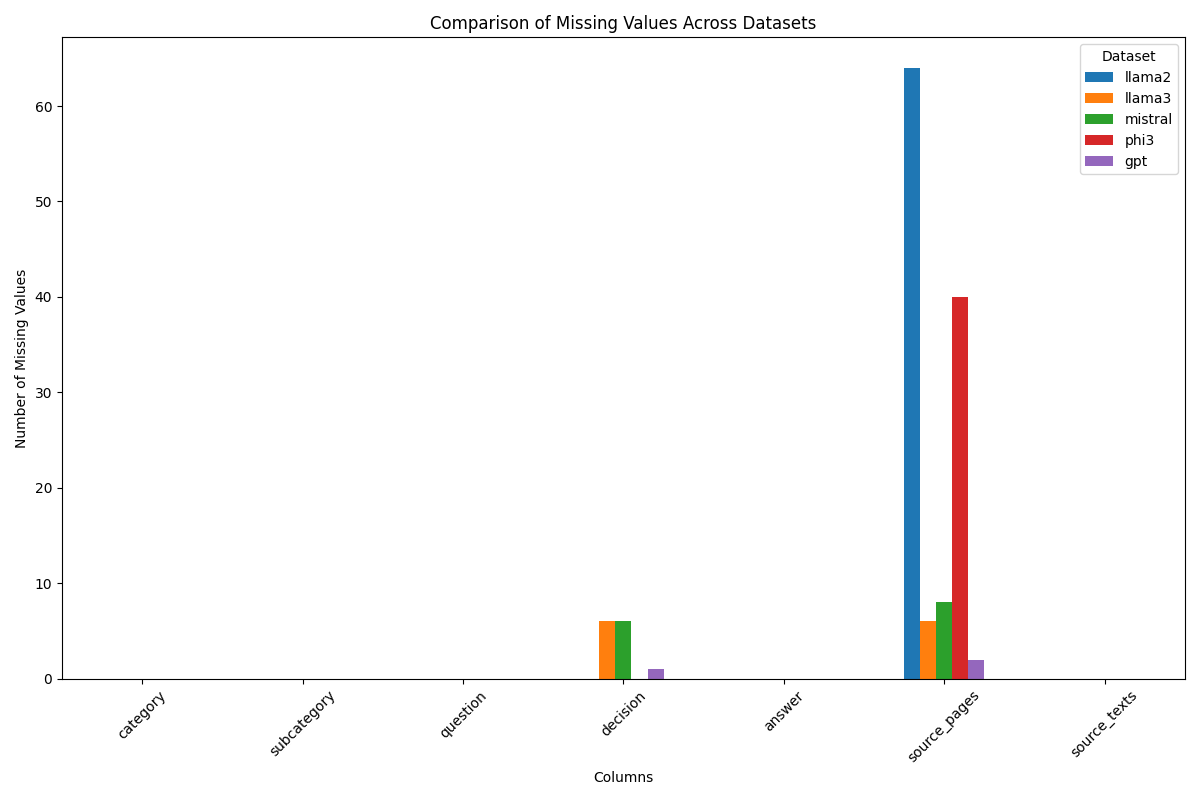
\includegraphics[width=0.8\textwidth]{./images/Missing_Values.png}
    \caption{Comparison of Missing Values Across Models}
    \label{fig:image_label}
\end{figure}

\textbf{Decision Metrics:} The first notable observation in the analysis of decisions pertains to the Llama2 model, 
which consistently answered "yes" to all questions. In contrast, 
the Mistral model displayed an approximately balanced response rate, with nearly 50\% of 
answers being "yes" and 50\% being "no." The Llama3 and Phi3 models produced more realistic outcomes, 
as both provided a higher proportion of "no" responses compared to "yes." Among these, 
the Mistral model exhibited a slight preference for "no" responses over the Llama3 model.
\newline\newline
An analysis of the missing decision entries for the Llama3 and Mistral models reveals the following patterns: 
in the case of the Llama3 model, three missing decisions are from the "target" category, 
two from the "strategy" category, and one from the "tracking" category. \newline
For the Mistral model, both the "strategy" and "tracking" categories have two missing entries each,
while the "target" and "governance" categories have one missing entry each. Notably, 
both models failed to provide an answer for question 36.
\newline\newline
\textbf{Source Page Metrics:} The majority of questions with missing source pages from the Llama3, Mistral, and Phi3 models 
fall within the "strategy" and "tracking" categories. 
Both the Llama3 and Mistral models fail to cite source pages for question 36. 
Additionally, Llama3 and Phi3 fail to provide source pages for questions 9, 19, 62, and 49, 
while Mistral and Phi3 fail to cite source pages for questions 34, 50, 37, and 63. Notably, 
there is no question for which all three models fail to provide a source page.
\newline\newline
\textbf{Disclosed indicators:} When comparing the "yes"-"no" counts of each model across different categories, 
the counts for Llama3 and Phi3 appear to be quite similar overall. However, 
a closer analysis of their counts within subcategories reveals subtle differences, 
particularly in the allocation of "yes" votes, 
while the "no" votes remain relatively consistent between the two models.

\subsubsection{H$\&$M}
\textbf{Missing Data:} An analysis of the H$\&$M missing responses shows that the Mistral model failed to answer 
five questions. Similar to the Zara report, 
all models struggled with citing source pages. 
The Llama3 model remained the best-performing in this aspect, with only three missing citations, 
while the Llama2 model once again failed to provide any source page citations. 
The Mistral model performed worse compared to the Zara report, 
with seven missing citations this time. 
The Phi3 model also showed a slight decline, failing to cite source pages for 43 entries.
\newline\newline

\textbf{Decision Metrics:}
Once again, the Llama2 model exclusively answered "yes," 
while the Mistral model maintained an approximately 50\% "yes"-"no" response rate. 
The Llama3 and Phi3 models exhibited response ratios similar to those observed in the Zara report. 
As before, the "target" category accounted for the highest number of missing decisions.

\begin{figure}[H]
    \centering
    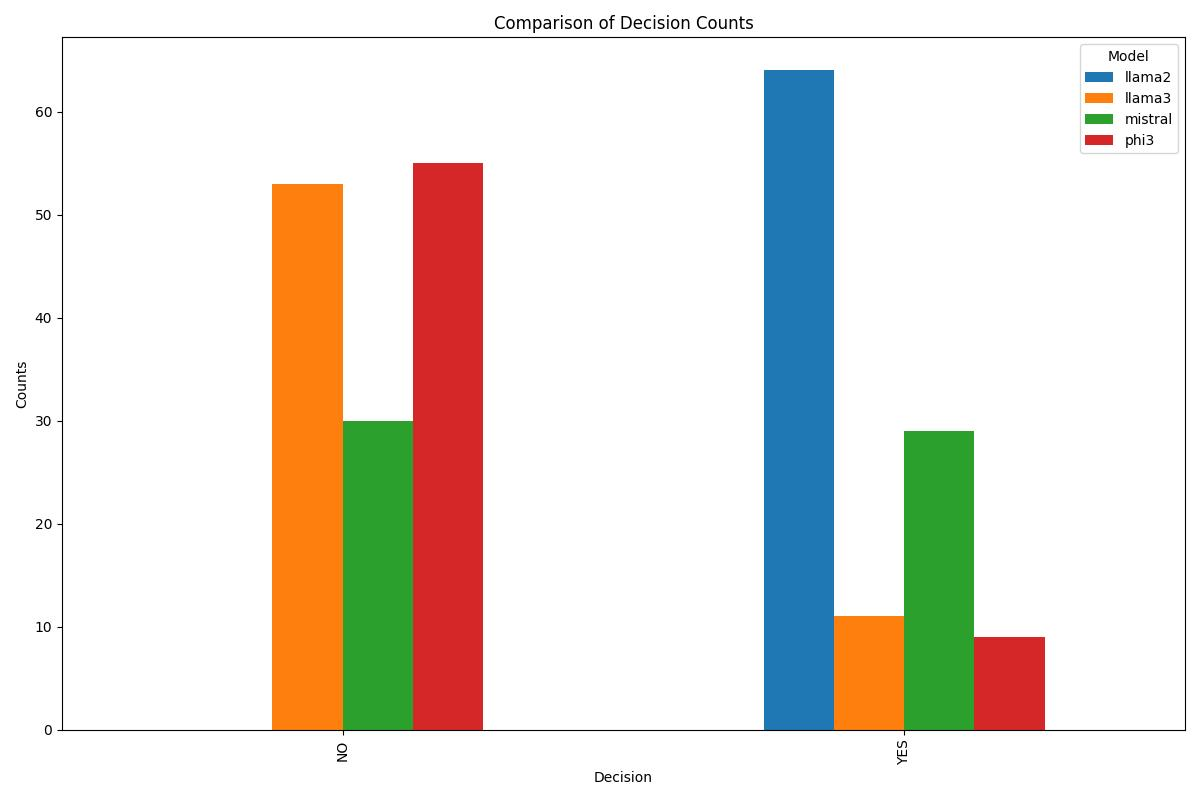
\includegraphics[width=0.8\textwidth]{./images/hm_comparison_decision.jpg}
    \caption{Comparison of Decision Counts Across Models}
    \label{fig:image_label}
\end{figure}

\textbf{Source Page Metrics:} The majority of questions with missing source pages from the Llama3, Mistral, 
and Phi3 models once again fall within the "strategy" and 
"tracking" categories. This time, the Llama3 and Mistral models do not have any overlap in their 
missing source pages. Both Llama3 and Phi3 fail to cite sources for questions 26 and 32, 
while Mistral and Phi3 fail to cite sources for questions 1, 10, 35, and 37. 
Notably, there is still no question for which all three models failed to provide a source page.
\newline\newline

\textbf{Disclosed indicators:} When comparing the "yes"-"no" counts of each model across different categories, 
the counts for Llama3 and Phi3 once again appear to be quite similar overall. However, 
a closer examination within subcategories reveals more pronounced differences compared to the Zara report. 
Meanwhile, the Mistral model continues to maintain an approximately 50-50 response rate across all categories.

\subsubsection{Conclusion}
Based on these quantitative evaluations we can conclude that all models face challenges in citing source pages, 
with Llama3 emerging as the most reliable in this aspect, and the persistent shortcomings of Llama2 in 
providing citations. Decision-making patterns highlighted distinct behaviors across models, 
with Llama2 consistently answering "yes," Mistral maintaining a balanced response ratio, 
and Llama3 and Phi3 demonstrating realistic response distributions. 
The "target" category repeatedly accounted for the highest number of missing decisions, 
and missing source pages were concentrated in the "strategy" and "tracking" categories. 
Despite these challenges, no single question was uniformly problematic across all models, 
underscoring the variability in model performance.


\section{Conclusions and Discussion} \label{sec:conclusions}

\begin{quotation}
    summarize the approach followed in this project and draw conclusions based on the results obtained
    \begin{itemize}
        \item Conclusions based on the approach followed and results obtained
        \item Discuss the meaning and findings of this project in a broader context considering the cluster selected and aim of this course
        \item Discuss limitations and future directions based on the findings obtained
    \end{itemize}
\end{quotation}

\printbibliography

\end{document}